\documentclass[12pt,letterpaper]{article}
\usepackage[margin=.63in,headheight=15pt,headsep=19pt,footskip=25pt]{geometry}
\usepackage{tikz,fancyhdr}
\usetikzlibrary{arrows.meta}
\renewcommand{\familydefault}{\sfdefault}
\pagestyle{fancy}\fancyhf{}\renewcommand{\headrulewidth}{.4pt}
\fancyhead[L]{\small Week 21 / Shortest routes encore / Grades 2--5}
\fancyfoot[L]{\small Bellingham Math Circle / Week 21 / W21-BON-v1}\fancyfoot[R]{\small\thepage}
\setlength{\parindent}{0pt}\setlength{\parskip}{8pt}
\newcommand{\problem}[2]{\textbf{Problem #1:} #2\par}
\newcommand{\routeboard}{\begin{tikzpicture}[x=20mm,y=20mm]
\draw[step=1,gray!25] (0,0) grid (8,8);\draw[thick] (0,1)--(8,1) (0,7)--(8,7);
\node[anchor=south east,font=\small,fill=white,inner sep=2pt] at (8,1){lower};\node[anchor=south east,font=\small,fill=white,inner sep=2pt] at (8,7){upper};
\fill (1,3) circle (2pt) node[above left]{A};\fill (7,5) circle (2pt) node[above right]{B};
\end{tikzpicture}}
\newcommand{\obstacleboard}[1]{\begin{tikzpicture}[x=20mm,y=20mm]
\draw[step=1,gray!25] (0,0) grid (8,8);\filldraw[fill=gray!18,draw=black,thick] (2,2) rectangle (6,5);
\fill (0,#1) circle (2pt) node[above right]{A};\fill (8,#1) circle (2pt) node[above left]{B};
\end{tikzpicture}}
\begin{document}
Use straight string pieces or a drawn route. Dot centers are endpoints. For the two-wall boards, stay between the walls, touch them in the stated order, and never travel along a wall.

\begin{center}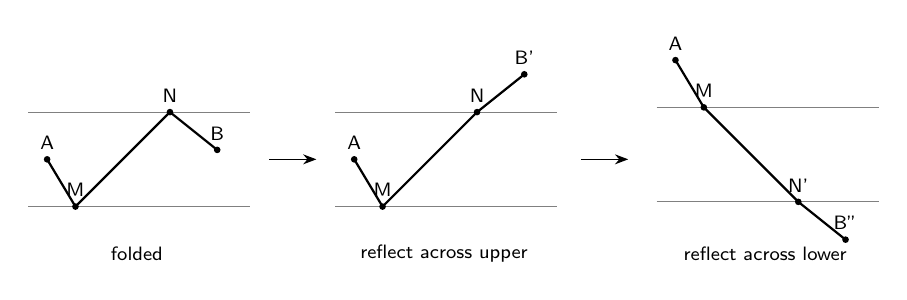
\begin{tikzpicture}[x=6mm,y=6mm]
\begin{scope}[shift={(0,0)}]
\draw[gray] (0,0)--(4.7,0) (0,2)--(4.7,2);\draw[thick] (.4,1)--(1,0)--(3,2)--(4,1.2);
\foreach \x/\y/\lab in {.4/1/A,1/0/M,3/2/N,4/1.2/B}{\fill (\x,\y) circle (1.2pt);\node[font=\scriptsize,above] at (\x,\y){\lab};}
\node[font=\scriptsize] at (2.3,-1){folded};\end{scope}
\draw[-{Stealth}] (5.1,1)--(6.1,1);
\begin{scope}[shift={(6.5,0)}]
\draw[gray] (0,0)--(4.7,0) (0,2)--(4.7,2);\draw[thick] (.4,1)--(1,0)--(3,2)--(4,2.8);
\foreach \x/\y/\lab in {.4/1/A,1/0/M,3/2/N,4/2.8/{B'}}{\fill (\x,\y) circle (1.2pt);\node[font=\scriptsize,above] at (\x,\y){\lab};}
\node[font=\scriptsize] at (2.3,-1){reflect across upper};\end{scope}
\draw[-{Stealth}] (11.7,1)--(12.7,1);
\begin{scope}[shift={(13.3,2.1)}]
\draw[gray] (0,0)--(4.7,0) (0,-2)--(4.7,-2);\draw[thick] (.4,1)--(1,0)--(3,-2)--(4,-2.8);
\foreach \x/\y/\lab in {.4/1/A,1/0/M,3/-2/{N'},4/-2.8/{B''}}{\fill (\x,\y) circle (1.2pt);\node[font=\scriptsize,above] at (\x,\y){\lab};}
\node[font=\scriptsize] at (2.3,-3.1){reflect across lower};\end{scope}
\end{tikzpicture}\end{center}

\problem{1}{Find the shortest route from A to B that touches the lower wall first and the upper wall second. Mark both contact points. Explain why a shorter legal route cannot work.}
\begin{center}\routeboard\end{center}
\newpage
\problem{2}{Find the shortest route from A to B that touches the upper wall first and the lower wall second. Which contact order gives a shorter route on this board?}
\begin{center}\routeboard\end{center}
\vspace{10pt}\hrulefill\par\vspace{12pt}\hrulefill
\newpage
For this board, touch the line exactly once, at a point in one of the two heavy windows. Window endpoints are allowed. Never travel along the line.

\problem{3}{Find the shortest allowed route from A to B. Decide which window it uses and where it touches. Explain why every other allowed contact gives a longer route.}
\begin{center}\begin{tikzpicture}[x=20mm,y=20mm]
\draw[step=1,gray!25] (0,0) grid (8,8);\draw (0,1)--(8,1);\draw[line width=3pt] (.5,1)--(2,1) (5,1)--(7.5,1);
\foreach \x in {.5,2,5,7.5}{\fill (\x,1) circle (2pt);}
\fill (1,3) circle (2pt) node[above left]{A};\fill (7,5) circle (2pt) node[above right]{B};
\end{tikzpicture}\end{center}
\vspace{10pt}\hrulefill\par\vspace{12pt}\hrulefill
\newpage
The shaded rectangle's interior is forbidden. Touching its edge or traveling along its edge is allowed.

\problem{4}{Find the shortest route from A to B around the rectangle. Explain why a route with different bends cannot be shorter.}
\begin{center}\obstacleboard{3}\end{center}
\vspace{10pt}\hrulefill\par\vspace{12pt}\hrulefill
\newpage
\problem{5}{Find every shortest route from A to B around this rectangle. Its interior is forbidden; its edge is allowed. Can different routes tie for the shortest length?}
\begin{center}\obstacleboard{3.5}\end{center}
\vspace{10pt}\hrulefill\par\vspace{12pt}\hrulefill
\end{document}
